\documentclass[aspectratio=169,xcolor=dvipsnames,t]{beamer}
\usepackage[utf8]{inputenc}

\usepackage{amssymb}
\usepackage{amsmath,bm}
\usepackage{rotating}
\usepackage{graphicx}
\usepackage[mathscr]{euscript}
\usepackage[dvipsnames,svgnames,table]{xcolor}
\usepackage{multicol}
\usepackage{multirow}
\usepackage{physics}
\usepackage[version=4]{mhchem}
\usepackage[spanish,es-nodecimaldot,es-tabla]{babel}
\usepackage{parskip}
\usepackage{hyperref}
\usepackage{csquotes}
\usepackage{wrapfig}
\usepackage{ragged2e}
\justifying

\usepackage{etoolbox}
\usepackage{textcase}
\makeatletter
\patchcmd{\beamer@Section}{\Section}{\Section{\MakeTextUppercase}{}{}}{}{}
\patchcmd{\beamer@Subsection}{\Subsection}{\Subsection{\MakeTextUppercase}{}{}}{}{}
\makeatother

\usepackage[backend=biber,citestyle=numeric-comp,bibstyle=apa,sorting=none]{biblatex}
\bibliography{ref}
\makeatletter
\RequireBibliographyStyle{numeric}
\makeatother

\newcommand{\be}{\begin{equation*}}
\newcommand{\ee}{\end{equation*}}
\newcommand{\ble}[1]{\begin{equation} \label{#1}}
\newcommand{\bae}{\begin{eqnarray}}
\newcommand{\eae}{\end{eqnarray}}
\newcommand{\pl}{\left(}
\newcommand{\pr}{\right)}
\newcommand{\kl}{\left[}
\newcommand{\kr}{\right]}
\definecolor{Grayo}{RGB}{72, 72, 72}
\definecolor{Graya}{RGB}{158, 158, 158}

\setbeamertemplate{footline}[frame number]

\usetheme{Arguelles}

%%%%%%%%%%%%%%%%%%%% Opciones título %%%%%%%%%%%%%%%

\title{Algoritmos de planificación del tratamiento: cálculos de dosis de fotones}
\subtitle{Khan's Treatment Planning in Radiation Oncology \tiny{\cite{Khans}}}

\date{\today}
\author{Christopher López Ruiz}
\institute{Instituto Nacional de Cancerología}

%%%%%%%%%%%%%%%%%%%%%%%%%%%%%%%%%%%%%%%%%%%%%%%%%%%%%%%%%%%%%%%%%%%

\begin{document}

\frame[plain,bg=fondo2.jpg]{\titlepage}

%%%%%%%%%%%%%%%%%%%%%%%%%%%%%%%%%%%%%%%%%%%

\Section{Introduccion}

\begin{frame}[standout]
      \centering\LARGE
      \textbf{\itshape\scshape Introducción}
\end{frame}

\begin{frame}

    \vspace{0.45cm}

    \begin{wrapfigure}{r}{0.3\textwidth}
        \centering
        \includegraphics[width=0.45\textwidth,angle=90]{tarjeta.jpg}
    \end{wrapfigure}

    \textbf{Historia}
    
    \begin{itemize}
        \item Los sistemas computarizados de planificación del tratamiento se han utilizado en la \textbf{planificación de la radioterapia desde la década de 1950}.
        \item El primer algoritmo informático utilizado se atribuyó a Tsien, quien \textbf{utilizó tarjetas perforadas para almacenar distribuciones de isodosis y permitir la adición de múltiples haces}.
        \item Los avances en la \textbf{velocidad de las computadoras y el desarrollo de algoritmos han mejorado} enormemente nuestra \textbf{capacidad para predecir las distribuciones de dosis de fotones en los pacientes}.
    \end{itemize}

\end{frame}

\begin{frame}
      
    En 1987 el \textbf{informe 42 de la ICRU} hace el primer intento de \textbf{clasificar los algoritmos de planificación informática}.

    \begin{figure}[h]
        \centering
        \includegraphics[width=0.6\textwidth]{tiposa.pdf}
    \end{figure}

    \textit{Empíricos}
    
    \begin{itemize}
        \item \textbf{Primeros algoritmos} se desarrollaron utilizando como \textbf{entrada datos de haces clínicos medidos en un phantom de agua plana.} Luego se hicieron \textbf{correcciones} para incorporar varios efectos.
        \item Con el tiempo, se incorporaron \textbf{factores de corrección de la heterogeneidad del paciente}, pero se aplicaron después, es decir, \textbf{después de realizar cálculos basados en agua asumiendo una geometría homogénea del paciente}.
    \end{itemize}

\end{frame}

\begin{frame}
    
    \begin{itemize}
        \item La mayor parte de este desarrollo se produjo \textbf{antes de la llegada de la CT}.
        \item Con el tiempo, la \textbf{utilización comercial de algoritmos empíricos se desvaneció.}
    \end{itemize}

    \begin{wrapfigure}{l}{0.4\textwidth}
        \centering
        \includegraphics[width=0.4\textwidth]{ct.jpeg}
    \end{wrapfigure}

    \textit{Basados en modelos}

    \begin{itemize}
        \item En \textbf{1990}, la \textbf{radioterapia conformada tridimensional (3D CRT) comenzó a utilizar datos de imágenes de CT} específicos del paciente en el proceso de planificación.
        \item Al principio \textbf{se limitaba a una simulación virtual}. Ya que \textbf{aún no estaban disponibles algoritmos informáticos} que pudieran incorporar la \textbf{información de densidad volumétrica} y calcular \textbf{distribuciones de dosis} tridimensionales en un período de tiempo razonable.
    \end{itemize}
\end{frame}

\begin{frame}

    \vspace{0.6cm}

    \begin{itemize}
        \item Para utilizar plenamente esta nueva información, fue necesario \textbf{desarrollar nuevos algoritmos que pudieran incorporar con mayor precisión variaciones en la anatomía de cada paciente}.
        \item Como resultado, los \textbf{sistemas comerciales de planificación de tratamientos han pasado a métodos de cálculo de fotones basados en modelos.}
    \end{itemize}

    \vspace{5pt}

    En este capítulo, se describen \textbf{tres modelos de cálculo de fotones que se utilizan actualmente en clínicas de radioterapia}. 
    
    Los modelos de cálculo de fotones son \textbf{un área de desarrollo continuo y es probable que la implementación de uno o más de estos modelos por parte de cada proveedor comercial difiera en muchos aspectos}. Sin embargo, la intención es \textbf{proporcionar una comprensión básica de los principios detrás de estos algoritmos}.

\end{frame}

%%%%%%%%%%%%%%%%%%%%%%%%%%%%%%%%%%%%%%%

\Section{La representacion del paciente}

\begin{frame}[standout]
      \centering\LARGE
      \textbf{\itshape\scshape La representación del paciente para la planificación de la dosis}
\end{frame}

\begin{frame}

    \textbf{Inicialmente}, los pacientes eran considerados como un \textbf{phantom de agua plana} con un \textbf{SSD} y una \textbf{profundidad específicos} para su uso en \textbf{cálculos de dosis simples o de unidades de monitorización}.

    El desarrollo de \textbf{herramientas de contorno externo} ayudó al planificador del tratamiento a determinar \textbf{distribuciones de dosis específicas para el paciente}. Dichos procedimientos dieron como resultado que el \textbf{paciente fuera representado como una composición homogénea} (es decir, agua), pero \textbf{permitieron la aplicación de correcciones superficiales al cálculo}.

    \begin{figure}[h]
        \centering
        \includegraphics[width=0.55\textwidth]{p1.pdf}
    \end{figure}

\end{frame}

\begin{frame}

    Las \textbf{heterogeneidades} de los pacientes \textbf{podrían representarse} de formas sencillas, como \textbf{utilizando contornos internos con densidades asignadas}.

    La densidad electrónica a asignar a la región podría \textbf{inferirse de los atlas de CT} o, si están disponibles, del \textbf{número medio de CT específico del paciente dentro de la estructura contorneada}.

    El \textbf{problema} con este enfoque fue que \textbf{tejidos} como el pulmón y el hueso \textbf{no son homogéneos en sí mismos y sus variaciones de densidad no se tendrían en cuenta al utilizar este enfoque}.

    \vspace{0.35cm}

    \begin{figure}[h]
        \centering
        \includegraphics[width=0.7\textwidth]{p2.pdf}
    \end{figure}

\end{frame}

\begin{frame}

    Todos los \textbf{sistemas de radioterapia modernos utilizan datos de imágenes volumétricas} para caracterizar al paciente en una \textbf{descripción 3D vóxel por vóxel}.
    
    El \textbf{conjunto de datos de imágenes más común utilizado} para la planificación es una \textbf{CT de planificación del tratamiento}, obtenida utilizando un \textbf{simulador de CT convencional}.

    Este conjunto \textbf{constituye la representación más precisa del paciente aplicable para el cálculo de dosis}, debido a la \textbf{relación uno a uno entre el número de CT y la densidad física y/o electrónica}.

    La \textbf{confiabilidad espacial de los escáneres de CT suele estar dentro del 2\%}, lo que genera \textbf{incertidumbres de dosis de aproximadamente el 1\%}.

    \begin{itemize}
        \item \textit{CBCT:} proporciona información sobre la alineación del paciente, pero la dispersión contenida en las imágenes dificulta la determinación precisa de la densidad.
        \item  \textit{MRI:} puede proporcionar un contraste tisular superior, pero la información en no está fuertemente relacionada con la densidad electrónica. Y es más propensa a artefactos.
    \end{itemize}

\end{frame}

\begin{frame}

    Además de la densidad electrónica, también \textbf{es necesario determinar la composición del tejido para algoritmos de cálculo más modernos}.

    En los algoritmos de \textbf{convolución/superposición}, las \textbf{tablas de atenuación de fluencia} normalmente se \textbf{calculan utilizando datos de coeficientes de atenuación de masa}, que dependen algo débilmente del material. 
    
    A menudo, estos \textbf{coeficientes se determinan para cada vóxel interpolando linealmente entre los resultados publicados de dos materiales diferentes} (por ejemplo, agua y hueso) en función de la \textbf{densidad asignada al vóxel}.
    
    Tanto para los cálculos de transporte de \textbf{MC} como de \textbf{Boltzmann}, se debe realizar una \textbf{asignación de material completa} para permitir una \textbf{determinación precisa de la sección transversal para el transporte de fotones y electrones} en todo el volumen del paciente.

    Idealmente, el \textbf{tamaño de los vóxeles en la CT de planificación del tratamiento} debería estar \textbf{cerca de la resolución de la cuadrícula de dosis utilizada para el cálculo}.

\end{frame}

%%%%%%%%%%%%%%%%%%%%%%%%%%%%%%%%%%%%%%%%%%%%%%%

\Section{Fisica basica de la radiacion}

\begin{frame}[standout]
    \centering\LARGE
    \textbf{\itshape\scshape Física básica de la radiación para el cálculo de dosis del haz de fotones}
\end{frame}

\begin{frame}

    \frametitle{Producción de fotones de megavoltaje}

    \vspace{-0.7cm}

    \begin{wrapfigure}{l}{0.36\textwidth}
        \centering
        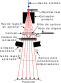
\includegraphics[width=0.36\textwidth]{linac.pdf}
    \end{wrapfigure}

    $\quad$

    \vspace{-0.1cm}

    \textbf{Acelerador lineal}, que consta de un \textbf{material de protección de alta densidad}, como plomo. 

    \textbf{Electrones de alta energía se aceleran} en la estructura aceleradora del linac e \textbf{inciden en el objetivo de rayos X} producción \textbf{radiación de frenado} (Bremsstrahlung).
    
    El tamaño del \textbf{punto focal de los electrones en el objetivo es pequeño}, típicamente del orden de unos pocos milímetros. Este tamaño finito \textbf{contribuye a la penumbra, o al desenfoque del haz cerca de los bordes del campo}.

    El \textbf{colimador primario} (aleación de tungsteno) \textbf{define el tamaño máximo del campo} que se puede utilizar para el tratamiento.

\end{frame}

\begin{frame}

    \vspace{-0.3cm}

    \begin{wrapfigure}{l}{0.36\textwidth}
        \centering
        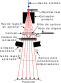
\includegraphics[width=0.36\textwidth]{linac.pdf}
    \end{wrapfigure}

    $\quad$

    \vspace{-0.3cm}

    En el caso de \textbf{energías de megavoltaje}, la \textbf{radiación de frenado se produce principalmente en dirección directa}.

    En la \textbf{mayoría de los aceleradores de arco en C convencionales}, para hacer que la \textbf{intensidad del haz sea más uniforme}, se coloca un \textbf{filtro cónico} en el haz.

    La \textbf{presencia del filtro de aplanado altera el espectro energético}, ya que el haz que atraviesa la parte central más gruesa del filtro tiene una mayor proporción de fotones de baja energía absorbidos.

    Es posible que esto \textbf{no sea necesario para la administración de tratamientos modernos} donde se utiliza \textbf{modulación para variar la intensidad del haz}, muchas unidades tienen la opción de quitar el filtro (\textbf{TrueBeam}).

\end{frame}

\begin{frame}

    \frametitle{Dispersión Compton}

    Los \textbf{fotones pueden dispersarse} inelásticamente mediante \textbf{tres procesos principales}:

    \begin{figure}
        \centering
        \includegraphics[width=0.9\textwidth]{efectos.pdf}
    \end{figure}

    En el \textbf{rango de energía utilizado para la radioterapia}, la \textbf{mayoría de las interacciones} son eventos de \textbf{dispersión Compton}.

\end{frame}

\begin{frame}

    Los \textbf{fotones dispersos Compton} pueden \textbf{originarse en el cabezal de tratamiento del acelerador} o en el \textbf{paciente (o phantom)}.

    La mayor parte de la dosis de dispersión generada por el \textbf{cabezal del acelerador se produce dentro del colimador primario y el filtro de aplanamiento de campo}. Estos fotones y electrones dispersos a veces se le denomina \textbf{``radiación extrafocal"}.

    \begin{wrapfigure}{r}{0.3\textwidth}
        \centering
        \includegraphics[width=0.3\textwidth]{comp.pdf}
    \end{wrapfigure}

    Para la dispersión generada por el \textbf{phantom}, las \textbf{características de penetración del haz también se modifican}. \textbf{A medida que aumenta el tamaño del campo, la dispersión del phantom hace que el haz sea significativamente más penetrante con la profundidad}.

    Este efecto es lo \textbf{suficientemente significativo} como para que esta \textbf{diferencia de energía deba incluirse en los cálculos de dosis}. 
    
    El comportamiento de la \textbf{dispersión de los modificadores del haz, como las cuñas, también debe considerarse dentro del modelo de fotones}.

\end{frame}

\begin{frame}

    \frametitle{Transporte de electrones}

    \textbf{Los fotones son radiación indirectamente ionizante}. La \textbf{dosis es depositada por partículas cargadas} puestas en movimiento desde el lugar de interacción del fotón.

    En \textbf{energías de megavoltaje}, el \textbf{alcance de las partículas cargadas puede ser de varios centímetros}. Estas partículas se mueven principalmente \textbf{hacia adelante}, pero se \textbf{dispersan considerablemente} a medida que \textbf{disminuyen su velocidad} y se \textbf{detienen}.

    \textbf{Los electrones pierden energía por dos procesos}:

    \begin{figure}
        \centering
        \includegraphics[width=0.85\textwidth]{pc.pdf}
    \end{figure}

\end{frame}

\begin{frame}

    La \textbf{naturaleza indirecta de la deposición de dosis de fotones} da como resultado varias \textbf{características en las distribuciones de dosis}.

    \begin{wrapfigure}{l}{0.28\textwidth}
        \centering
        \includegraphics[width=0.28\textwidth]{pdd.pdf}
    \end{wrapfigure}

    La \textbf{dosis superficial aumenta (se “acumula”) desde la superficie del paciente debido al mayor número de PC (partículas cargadas) que se ponen en movimiento}. Esto da como resultado una \textbf{dosis cutánea baja}, cuya magnitud es inversamente proporcional a la longitud del camino de las PC.

    La \textbf{dosis aumenta hasta un máximo a una profundidad}, $D_{max}$,característica de la energía del haz de fotones. 

    En un punto del paciente con una \textbf{profundidad igual a la distancia de penetración de las PC}, las \textbf{PC que se detienen se reponen con PC que se ponen en movimiento} y se dice que se alcanza el \textbf{equilibrio de partículas cargadas (CPE)}.

    En este caso, la \textbf{dosis en un punto es proporcional a la fluencia de energía de los fotones en el mismo punto}. 

\end{frame}

\begin{frame}

    \vspace{0.3cm}

    \begin{wrapfigure}{r}{0.28\textwidth}
        \centering
        \includegraphics[width=0.28\textwidth]{ee.pdf}
    \end{wrapfigure}

    El \textbf{criterio principal para CPE es que la fluencia de energía de los fotones debe ser constante en el rango de electrones puestos en movimiento en todas las direcciones}. En general, esto \textbf{no ocurre en medios heterogéneos}, cerca del límite del haz o en haces de intensidad modulada. 

    Los \textbf{electrones producidos en la cabeza del acelerador y en el aire entre el acelerador y el paciente se denominan \textit{electrones de contaminación}}.
    
    La \textbf{interacción de estos electrones} dentro y justo más allá de la región de acumulación \textbf{contribuye significativamente a la dosis, especialmente si el campo es grande}.
    
    La \textbf{perturbación en el transporte de electrones puede exagerarse cerca de las heterogeneidades}.

\end{frame}


%%%%%%%%%%%%%%%%%%%%%%%%%%%%

\Section{Algoritmo de superposicion/convolucion}

\begin{frame}[standout]
    \centering\LARGE
    \textbf{\itshape\scshape Algoritmo de superposición/convolución}
\end{frame}

\begin{frame}

    Es el \textbf{cálculo de dosis de fotones más común} que se utiliza hoy en día para la planificación de radioterapia.

    Este método \textbf{incorpora un enfoque basado en modelos} para describir la física subyacente de las interacciones, sin dejar de poder \textbf{calcular la dosis en un tiempo razonable}.

    Este \textbf{comienza modelando la naturaleza indirecta de la deposición de dosis a partir de haces de fotones}.
    
    Las \textbf{interacciones de los fotones primarios se tratan por separado del transporte de fotones dispersos y electrones puestos en movimiento}.

    \begin{figure}
        \centering
        \includegraphics[width=0.48\textwidth]{CS.pdf}
    \end{figure}

\end{frame}

\begin{frame}

    \frametitle{Cálculo de dosis en condiciones de equilibrio de partícula cargada}

    Consideramos \textbf{el caso especial de la determinación de dosis en condiciones de CPE}. 

    En este caso, \textbf{la energía total absorbida por las partículas cargadas} en la posición $r$ \textbf{es la misma que la energía total que escapa} debido a las interacciones de los fotones en el mismo lugar.

    Por tanto, \textbf{la dosis primaria $D_P$ y la primera dosis dispersada de un haz paralelo de fotones monoenergéticos se pueden calcular como}:

    \bae \label{Dp}
    \begin{split}
    D_P(\mathbf{r}) = \pl K_c(\mathbf{r}) \pr_P = \pl \frac{\mu_{en}}{\rho} \pr_P \psi_{P} (\mathbf{r}) \\
    \quad \quad \quad \, \, \, = \pl \frac{\mu_{en}}{\rho} \pr_P \phi_{P} (\mathbf{r}=0) \, h\nu_P \, e^{-\mu r}
    \end{split}
    \eae
    
\end{frame}

\begin{frame}

    \vspace{-0.2cm}

    \be
    D_P(\mathbf{r}) = \pl K_c(\mathbf{r}) \pr_P = \pl \frac{\mu_{en}}{\rho} \pr_P \psi_{P} (\mathbf{r})
    \ee
    \be
    \quad \quad \quad \, \, \, = \pl \frac{\mu_{en}}{\rho} \pr_P \phi_{P} (\mathbf{r}=0) \, h\nu_P \, e^{-\mu r} 
    \ee

    Donde:

    \vspace{-0.6cm}

    \be
    \pl K_c(\mathbf{r}) \pr_P = \text{kerma de colisión},
    \ee
    \be
    \pl \frac{\mu_{en}}{\rho} \pr = \text{coeficiente másico de absorción de energía}, 
    \ee
    \be
    \psi_{P} (\mathbf{r}) = \text{fluencia de energía primaria},
    \ee
    \be
    \phi_{P} (\mathbf{r}=0) = \text{fluencia de fotones primarios en la superficie del phantom},
    \ee
    \be
    h\nu_P = \text{energía del fotón primario}, 
    \ee
    \be
    \mu = \text{coeficiente de atenuación de fotones primarios}
    \ee

\end{frame}

\begin{frame}

    La \textbf{dosis total es la suma de los componentes primario y disperso}.

    \bae
    D_{tot}(\mathbf{r}) = D_P(\mathbf{r}) + \int D_P(\mathbf{r'}) \frac{\pl \mu_{en} \pr_{scat} \pl h\nu \pr_{scat}}{\pl \mu_{en} \pr_{P} \pl h\nu \pr_{P}} \derivative{P_{scat} (\theta,\mathbf{r'})}{V} e^{-\mu_{scat}(r'-r)} \text{d}V
    \eae
    
    Donde $\derivative{P_{scat} (\theta,\mathbf{r'})}{V}$ es la probabilidad por unidad de volumen de que un fotón primario se disperse en un ángulo sólido centrado alrededor del ángulo $\theta$.

    Estas \textbf{no tienen en cuenta ninguna dispersión de fotones secundarios o de orden superior}.

    También \textbf{ignoran la divergencia del haz} y \textbf{no tienen en cuenta las heterogeneidades de los tejidos}. Son \textbf{válidos sólo para situaciones de CPE}, de modo que el \textbf{cálculo de la dosis no es válido en la región de acumulación o cerca de los límites del campo}, y la \textbf{dosis dispersa se ve perturbada por las heterogeneidades que se encuentran entre el sitio de dispersión en $r'$ y el punto $r$, donde la dosis total se está calculando}.

\end{frame}

\begin{frame}

    \frametitle{Método de convolución/superposición}

    Desafortunadamente, \textbf{la ecuación} \eqref{Dp} \textbf{es simplista} porque \textbf{no tiene en cuenta el alcance finito de partículas cargadas}, $\rightarrow$ \textbf{la fluencia de energía que estaba presente en el punto en que las partículas cargadas se pusieron en movimiento debería reemplazar la fluencia de energía en la ecuación} \eqref{Dp}.

    En realidad, \textbf{las partículas pueden originarse en cualquier ubicación alrededor del punto de cálculo, siempre que esté dentro del alcance de partículas}.

    Por lo tanto, en lugar de un \textbf{único sitio de interacción de fotones efectivo}, esta expresión para la dosis \textbf{se convierte en una integral de convolución alrededor de $r$}:

    \bae \label{DPc}
    D(\mathbf{r}) = \int K_c(\mathbf{r'}) A_c (\mathbf{r}-\mathbf{r'}) \text{d}\mathbf{r'}
    \eae
    
\end{frame}

\begin{frame}
    
    \vspace{0.5cm}

    \be
    D(\mathbf{r}) = \int K_c(\mathbf{r'}) A_c (\mathbf{r}-\mathbf{r'}) \text{d}\mathbf{r'}
    \ee

    Donde $A_c (\mathbf{r}-\mathbf{r'})$ describe la \textbf{contribución de la energía de las partículas cargadas} que se absorbe por unidad de volumen en $\mathbf{r}$ a partir de interacciones en $\mathbf{r'}$ y la integración es sobre todos los valores de $\mathbf{r'}$ que componen el volumen d$\mathbf{r'}$.

    La \textbf{ecuación \eqref{DPc} requiere conocimiento de la fluencia de energía debida a los fotones primarios y dispersos en todos los puntos}.Para esto \textbf{se necesitarían métodos de transporte que consumirían mucho tiempo} para calcular con precisión el componente disperso.

    Una \textbf{solución más sencilla} es utilizar un \textbf{núcleo de dispersión que incluya el componente de fotones dispersos junto con la contribución de las partículas cargadas}. 
    
\end{frame}

\begin{frame}

    \vspace{0.5cm}
    
    El \textbf{núcleo ya no es finito} porque se incluye la dispersión de fotones (que no tiene alcance). Ahora \textbf{sólo se transportan explícitamente fotones primarios}. 
    
    Una \textbf{ecuación de convolución que separa el transporte de fotones primarios} y un \textbf{núcleo que explica los fotones y electrones dispersos puestos en movimiento lejos del sitio de interacción del fotón primario es la siguiente}:
    
    \bae
    D(\mathbf{r}) = \int \frac{\mu}{\rho} \psi_P(\mathbf{r'}) A_c (\mathbf{r}-\mathbf{r'}) \text{d}\mathbf{r'} = \int T_P(\mathbf{r'}) A_c (\mathbf{r}-\mathbf{r'}) \text{d}\mathbf{r'}
    \eae

    El producto del \textbf{coeficiente másico de atenuación} y la \textbf{fluencia de energía primaria} es la \textbf{terma primaria} (\textit{total energy released per unit mass}) $T_P(\mathbf{r'})$.
    
\end{frame}

\begin{frame}

    En principio, los \textbf{núcleos de convolución pueden obtenerse mediante cálculo analítico}, \textbf{deconvolución a partir de distribuciones de dosis} o incluso mediante \textbf{medición directa}. 
    
    Muy a menudo, los núcleos se \textbf{calculan con el método MC} haciendo \textbf{interactuar una gran cantidad de fotones primarios en un lugar} y determinando de \textbf{dónde se absorbe la energía}, es decir, de las \textbf{partículas cargadas generadas primariamente}, las \textbf{partículas cargadas que posteriormente se ponen en movimiento a partir de fotones dispersos o ambos}.

    \begin{figure}
        \centering
        \includegraphics[width=0.4\textwidth]{ruleta.jpg}
    \end{figure}
    
\end{frame}

\begin{frame}

    \begin{wrapfigure}{l}{0.28\textwidth}
        \centering
        \includegraphics[width=0.28\textwidth]{f1.jpg}
    \end{wrapfigure}

    \textbf{Núcleos de cobalto-60} (fotones primarios de 1.25 MeV) para agua calculados mediante simulación de Monte Carlo. Las líneas de isovalor están en unidades de $cGy$ $MeV^{-1}$ fotón$^{-1}$. 
    
    \textbf{A:} La contribución debida a los electrones puestos en movimiento a partir de fotones primarios (es decir, la contribución primaria). 
    
    \textbf{B:} La primera contribución de dispersión. 
    
    \textbf{C:} La suma de las contribuciones primarias y todas las de dispersión.

    El \textbf{núcleo está dirigido hacia adelante} incluso con esta energía baja. A medida que \textbf{aumenta la energía, el núcleo se vuelve aún más puntiagudo}.
    
\end{frame}

\begin{frame}

    \frametitle{Modelado de fotones primarios incidentes en el phantom}

    La \textbf{ecuación de convolución se limita a describir haces paralelos monoenergéticos de fotones primarios que interactúan con phantoms homogéneos}.

    En la actualidad, la \textbf{información espectral se deriva de simulaciones de MC comparadas mediante medición}. 
    
    Utilizando el método \textbf{MC EGS4}, Mohan y Chui \textbf{cuantificaron por primera vez el espectro de aceleradores clínicos utilizando el método MC}. Desde entonces, varios \textbf{otros autores han realizado simulaciones para calcular el espectro de energía de los fotones}.

    \textbf{Se esperaría que el espectro también variara con la posición fuera del eje si se utiliza un filtro de aplanado de campo}.

\end{frame}

\begin{frame}

    Tenemos la \textbf{distribución media de energía de fotones} en un campo abierto de $40 \times 40 \, cm$  desde un \textbf{objetivo de haz de fotones} de 10 $MV$, un \textbf{colimador primario} y un \textbf{filtro de aplanado de campo}. Equipo  Varian 2100C. Los valores corresponden a fotones en el aire que llegan al plano del isocentro.

    \begin{wrapfigure}{l}{0.48\textwidth}
        \centering
        \includegraphics[width=0.48\textwidth]{f2.jpg}
    \end{wrapfigure}

    La figura muestra que \textbf{la energía media de la radiación primaria} (directamente desde el objetivo) \textbf{disminuye fuera del eje, pero los fotones extrafocales} (colimador primario y filtro de aplanado) \textbf{no lo hacen}. 

    Esta disminución fuera del eje \textbf{se debe al endurecimiento diferencial del haz por el filtro de aplanado}. Dado que \textbf{domina el componente fotónico directo}, el \textbf{modelo debe tener en cuenta el cambio en el espectro de energía a lo largo del campo}.
    
\end{frame}

\begin{frame}

    Los \textbf{colimadores y los contornos del campo de bloques} generalmente se \textbf{modelan con una función de máscara matemática}, que consiste en la \textbf{fracción de la fluencia incidente transmitida a través del modificador}. 

    Para un \textbf{colimador}, la función de máscara dentro del campo es la \textbf{unidad}, y \textbf{debajo del colimador es igual a la transmisión del colimador primario}. 
    
    Para un \textbf{bloque}, la función de máscara dentro del campo es la \textbf{transmisión primaria a través de la bandeja del bloque}, y \textbf{debajo del bloque es igual a la transmisión del bloque primario}.

    \be
    A \rightarrow A \times B \rightarrow A \times B \times C
    \ee

    La \textbf{función de máscara por sí sola no sería capaz de modelar el desenfoque penumbral del límite del campo}. Esto ha sido modelado mediante una \textbf{función de apertura}. 

\end{frame}

\begin{frame}

    Las \textbf{cuñas y compensadores convencionales no se pueden modelar con precisión únicamente con atenuación primaria}.

    Estos componentes producen \textbf{dispersión y provocan un endurecimiento diferencial del haz}, este último se puede \textbf{contabilizar según el material de la cuña y el espectro del haz en función de la posición radial}. 

    La \textbf{dispersión de la cuña es más difícil de explicar}. La \textbf{mayor dispersión hace que el factor de cuña aumente en un pequeño porcentaje en función del tamaño del campo}. Esto puede \textbf{modelarse adecuadamente mediante un factor dependiente del tamaño del campo que duplique el efecto}.
    
    Alternativamente, \textbf{se puede incluir la cuña o el compensador como parte de la representación del paciente}. Este \textbf{phantom extendido} tiene una \textbf{gran heterogeneidad}, es decir, \textbf{el espacio de aire entre el dispositivo y el paciente}. Este método puede predecir la variación del factor de cuña en función del tamaño del campo.

\end{frame}

\begin{frame}

    \frametitle{Seguimiento de rayos de la fluencia de la energía incidente a través del phantom}

    \begin{wrapfigure}{l}{0.26\textwidth}
        \centering
        \includegraphics[width=0.26\textwidth]{f3.jpg}
    \end{wrapfigure}

    La \textbf{distribución de fluencia de energía 2D incidente se traza con rayos a través del paciente para crear una distribución de fluencia de energía 3D}.

    La \textbf{densidad de los rayos seguidos y el muestreo de los rayos} a lo largo de su trayectoria \textbf{deben ser suficientes para representar el comportamiento de atenuación del phantom}. 
    
    Una \textbf{densidad de muestreo suficiente es especialmente importante para los campos tangenciales de cabeza, cuello y mama}. 
    
    En general, la \textbf{densidad de muestreo requerida es mayor que la resolución de dosis deseada}, por lo que \textbf{varios rayos atraviesan cada vóxel de cálculo}.

\end{frame}

\begin{frame}

    Ya con lo anterior ...

    \textbf{Terma se calcula dentro de la matriz de cálculo multiplicando la fluencia primaria por el coeficiente de atenuación de masa}. 
    
    El \textbf{coeficiente de atenuación del rayo primario}, ponderado según el espectro del haz apropiado, \textbf{se basa en las propiedades del vóxel}. 
    
    La \textbf{fluencia de energía en un punto de muestra se reduce con respecto a la muestra anterior a lo largo del rayo}. 
    
    El \textbf{endurecimiento del espectro de fluencia de energía primaria con profundidad y posición fuera del eje se explica cambiando el coeficiente de atenuación con la posición}. 
    
    La \textbf{velocidad de la operación de trazado de rayos se puede mejorar significativamente mediante el uso de tablas de búsqueda para almacenar los resultados calculados previamente}.

\end{frame}

\begin{frame}

    \frametitle{Contaminación electrónica}

    \textbf{No se tiene en cuenta en el método de convolución convencional}, por lo que se debe \textbf{agregar un componente independiente adicional} para tener en cuenta esta dosis.

    \textbf{La dosis superficial de los haces de fotones de megavoltaje se debe casi en su totalidad al componente de contaminación electrónica}. 

    Estudios en los que la \textbf{contaminación electrónica se ha eliminado} mediante barrido magnético de electrones del campo revelan que \textbf{la dosis de los electrones contaminantes se asemeja a un haz de electrones con un alcance práctico algo mayor que la profundidad de la dosis máxima}.

    Se puede obtener una \textbf{concordancia razonable con las curvas PDD medidas escalando la curva de PDD de electrones de contaminación con la dosis de superficie} y \textbf{agregando este componente a la distribución de dosis calculada por convolución}.

\end{frame}

\begin{frame}

    \frametitle{Varianza espacial del núcleo y heterogeneidades del phantom}

    \be
    D(\mathbf{r}) \int T_P(\mathbf{r'}) A_c (\mathbf{r}-\mathbf{r'}) \text{d}\mathbf{r'}
    \ee

    La \textbf{ecuación de convolución supone que el núcleo es espacialmente invariante} en el sentido de que \textbf{el valor del núcleo depende sólo de la relación geométrica relativa entre los sitios de interacción y deposición de dosis} y \textbf{no de su posición absoluta en el phantom}.

    Cuando esto es \textbf{cierto, el cálculo de la convolución se puede realizar en el espacio de Fourier}, ahorrando mucho tiempo. Desafortunadamente, \textbf{este no es el caso ya que el núcleo varía según la posición}.

    Los \textbf{efectos del endurecimiento y la divergencia del haz son pequeños} y pueden \textbf{calcularse de varias formas}. 

\end{frame}

\begin{frame}

    Se puede utilizar una \textbf{corrección multiplicativa de la terma} en el paciente para corregir el endurecimiento del núcleo.

    Alternativamente, se pueden \textbf{utilizar varios núcleos válidos para diferentes profundidades} en el phantom como base para la \textbf{interpolación a una profundidad específica}. 

    Se ha demostrado que la \textbf{corrección en función de la profundidad es casi lineal}, y \textbf{no emplear ninguna corrección da como resultado una discrepancia de $\sim4\%$ a 30 $cm$ de profundidad}.

    \textbf{Las heterogeneidades fantasma son un problema más grave.}

    \textbf{Modelar el transporte de electrones y fotones dispersos a través de un fantasma heterogéneo requeriría un núcleo único en cada ubicación}. Cada núcleo se \textbf{superpondría} en la cuadrícula de dosis y se \textbf{ponderaría} con respecto al terma primario.

\end{frame}

\begin{frame}

    Lo que se requiere para que el cálculo sea manejable es \textbf{modificar un núcleo, calculado en un medio homogéneo, para que sea razonablemente representativo en una situación heterogénea}.

    Si la \textbf{mayor parte de la energía entre el sitio de interacción principal y el sitio de deposición de dosis se transporta en el camino directo entre estos sitios}, es posible tener una \textbf{corrección} relativamente simple \textbf{de la ecuación de convolución basada en el trazado de rayos entre los sitios de interacción y deposición de dosis}, y \textbf{escalar la longitud del camino por densidad} para obtener la \textbf{longitud del camino radiológico entre estos sitios}.

    La \textbf{ecuación de convolución modificada para la longitud del camino radiológico se llama ecuación de superposición}:

    \bae
    D(\mathbf{r}) \int T_P(\rho_{r'}\cdot \mathbf{r'}) A_c (\rho_{r'-r}\cdot (\mathbf{r}-\mathbf{r'})) \text{d}\mathbf{r'}
    \eae

\end{frame}

\begin{frame}

    \begin{wrapfigure}{r}{0.45\textwidth}
        \centering
        \includegraphics[width=0.35\textwidth]{dr.pdf}
    \end{wrapfigure}

    \be
    D(\mathbf{r}) \int T_P(\rho_{r'}\cdot \mathbf{r'}) A_c (\rho_{r'-r}\cdot (\mathbf{r}-\mathbf{r'})) \text{d}\mathbf{r'}
    \ee

    Donde:
    
    $\rho_{r'-r}\cdot (\mathbf{r}-\mathbf{r'})$ es la distancia radiológica desde el sitio de deposición de la dosis hasta el sitio de interacción del fotón primario.
    
    $\rho_{r'}\cdot \mathbf{r'}$ es la distancia radiológica desde la fuente hasta el sitio de interacción del fotón.

\end{frame}

\begin{frame}

    \begin{wrapfigure}{l}{0.29\textwidth}
        \centering
        \includegraphics[width=0.29\textwidth]{f4.jpg}
    \end{wrapfigure}

    Woo y Cunningham \textbf{compararon el núcleo modificado de fotones primarios de 6 $MeV$ generado por MC en un phantom de agua que contiene un anillo de aire}. 
    
    La \textbf{línea discontinua es un núcleo modificado para la situación heterogénea} utilizando una escala de rango a partir de uno \textbf{derivado en un phantom homogéneo}. La \textbf{línea continua es un núcleo calculado explícitamente para la situación heterogénea}.

    Los resultados mostrados indican que la \textbf{concordancia no es perfecta}, pero las tendencias computacionales son claramente evidentes en el sentido de que las \textbf{líneas de isovalor se contraen en regiones de alta densidad y se expanden en regiones de baja densidad}.

\end{frame}

%%%%%%%%%%%%%%%%%%%%%%%

\Section{Monte Carlo}

\begin{frame}[standout]
    \centering\LARGE
    \textbf{\itshape\scshape Monte Carlo}
\end{frame}

\begin{frame}

    La \textbf{técnica de transporte de radiación de Monte Carlo (MC)} consiste en \textbf{utilizar distribuciones de probabilidad bien establecidas} que rigen las interacciones individuales de electrones y fotones para \textbf{simular su transporte a través de la materia}.

    Aunque el método MC se había \textbf{propuesto desde hacía algún tiempo, no pudo utilizarse plenamente hasta el desarrollo de la computadora digital en la década de 1940}.

    El \textbf{transporte de radiación} fue uno de los \textbf{primeros usos de esta metodología} en ese momento, y los códigos públicos, como el \textbf{código de transporte de N partículas de Monte Carlo (MCNP)}, comenzaron a aparecer ya en la década de 1950.

    En los cálculos del transporte de fotones, el \textbf{código de transporte de electrones (ETRAN)}, desarrollado por la Oficina Nacional de Estándares en la década de 1970, \textbf{se basó en la técnica de historial condensado} introducida por primera vez por Berger en 1963.

    El código \textbf{Electron Gamma Shower (EGS4)} se desarrolló originalmente en el \textbf{Acelerador Lineal de Stanford en la década de 1980} y ahora lo mantiene (como EGSnrc modificado) el \textbf{Consejo Nacional de Investigación de Canadá}. 

\end{frame}

\begin{frame}

    \frametitle{Simulaciones análogas}

    Como señala el \textbf{TG 105}, una \textbf{simulación análoga} es la \textbf{propagación aleatoria de una partícula a través de los siguientes cuatro pasos}:

    \begin{enumerate}
        \item Determinar la distancia hasta la siguiente interacción.
        \item Transportar la partícula al sitio de interacción.
        \item Seleccionar qué interacción tendrá lugar.
        \item Simular esta interacción.
    \end{enumerate}

    El \textbf{paso inicial} se realiza en función de la \textbf{probabilidad de que la partícula interactúe dentro del medio en cuestión}.

\end{frame}

\begin{frame}

    Por ejemplo, si la \textbf{probabilidad de interacción está representada por un coeficiente de atenuación} $\mu$, se puede determinar una \textbf{distancia de interacción aleatoria} $r$ a partir de un \textbf{número aleatorio $\varepsilon$ (entre 0 y 1)} mediante lo siguiente:

    \vspace{-0.2cm}

    \bae
    r=-\frac{(1-\varepsilon)}{\mu}
    \eae

    \vspace{-0.2cm}

    El \textbf{segundo paso }es relativamente sencillo, pero se requiere conocimiento de la \textbf{densidad de masa} (y los cambios correspondientes en $\mu$) para \textbf{materiales heterogéneos}. 
    
    Se realizará otra \textbf{elección aleatoria para el paso 3}, \textbf{ponderada proporcionalmente a las probabilidades relativas de las opciones de interacción} (Compton, fotoeléctrico, pp). 
    
    \textbf{Finalmente} se deben \textbf{simular aleatoriamente los resultados de la interacción}, incluyendo las \textbf{partículas de nueva energía} (si no son absorbidas) y su \textbf{trayectoria}.

\end{frame}

\begin{frame}

    \frametitle{Historiales condensados}

    Si bien las \textbf{simulaciones análogas funcionan bien para las interacciones de fotones}, surge un \textbf{problema} práctico para el transporte de \textbf{electrones}.

    El \textbf{camino libre medio para los electrones en el rango de energía terapéutica es del orden de $10^{-5} \, g/cm^2$}. Esto significa que \textbf{un solo electrón de energía $>1 \, MeV$ tendrá más de 105 interacciones antes de detenerse}. Realizar una simulación análoga de este evento \textbf{no es práctico}.

    La \textbf{técnica del transporte de electrones de historial condensado} fue introducida por primera vez por \textbf{Berger en 1963}. Observó que \textbf{la mayoría de las interacciones inelásticas de electrones no perdían mucha energía ni tenían un cambio direccional significativo}.

    Estas \textbf{interacciones "suaves"} podrían \textbf{estar separadas por eventos "catastróficos" más significativos}, donde el electrón tuvo una \textbf{pérdida de energía significativa} (ejem., producción de rayos delta, evento Bremsstrahlung).

\end{frame}

\begin{frame}

    \vspace{1cm}

    Las \textbf{interacciones suaves} podrían \textbf{simularse por separado combinándolas en interacciones virtuales únicas de gran efecto}, mientras que los \textbf{eventos catastróficos pueden simularse de forma análoga} como se describió anteriormente.

    Para \textbf{electrones con energías superiores a un umbral de energía}, el camino libre medio para interacciones catastróficas es \textbf{varios órdenes de magnitud mayor}.

    Si bien este enfoque \textbf{permite cálculos más rápidos}, se ha demostrado que la elección del \textbf{tamaño de paso} para los historiales condensados produce \textbf{artefactos en los resultados}.
    
    Sin embargo, estos problemas han llevado a \textbf{métodos de historial condensado mejorados y de alta precisión}.

\end{frame}

\begin{frame}

    \frametitle{Técnicas de reducción de varianza}

    \textbf{ En lugar de simular eventos individuales} como en una simulación análoga, se pueden emplear \textbf{técnicas para mejorar la eficiencia del cálculo de MC para obtener un resultado particular}.

    \begin{wrapfigure}{l}{0.25\textwidth}
        \centering
        \includegraphics[width=0.25\textwidth]{var.pdf}
    \end{wrapfigure}

    Las \textbf{técnicas de reducción de la varianza} se utilizan para \textbf{reducir la varianza} de un resultado de cálculo determinado para un \textbf{número determinado de historiales}.

    Por ejemplo, una \textbf{simulación análoga de un evento Bremsstrahlung} seleccionaría aleatoriamente \textbf{una energía y una dirección} (proporcional a sus respectivas probabilidades) para la \textbf{emisión de fotones resultante}. 
    
    \textbf{Alternativamente, se podría simular la emisión de una gran cantidad de fotones con pesos más bajos} para \textbf{imitar mejor la emisión direccional aleatoria de estos eventos}.

\end{frame}

\begin{frame}

    Esta técnica particular se denomina \textbf{división Bremsstrahlung} y es una de las muchas técnicas diferentes que pueden emplearse dentro de un código MC particular. 
    
    Las \textbf{técnicas son importantes para mantener los tiempos de cálculo prácticos} en la mayoría de las situaciones. 

    Se debe \textbf{tener cuidado de que la física subyacente no esté sesgada por los resultados}.

    \vspace{0.2cm}

    \begin{figure}
        \centering
        \includegraphics[width=0.45\textwidth]{var.pdf}
    \end{figure}

\end{frame}

\begin{frame}

    \frametitle{Cálculos de dosis de radioterapia de Monte Carlo}

    En principio, \textbf{es posible simular historiales de toda la administración de radioterapia}, $\rightarrow$ desde el \textbf{impacto inicial del electrón acelerado sobre el objetivo hasta la dosis administrada}. 
    
    Sin embargo, este \textbf{sería un proceso tremendamente ineficaz}, ya que \textbf{pocos de estos historiales pasarían del acelerador hasta llegar al paciente}. 

    Alternativamente, \textbf{es posible transportar las partículas a través de estructuras independientes del paciente} (por ejemplo, objetivo, colimador primario, cámara de iones) y \textbf{almacenar esta información para uso futuro}. 

    \textbf{Esta información se conoce como archivo de espacio de fases} y contiene información que incluye la \textbf{posición, la energía y la dirección de los fotones y electrones emitidos por el acelerador}.

\end{frame}

\begin{frame}

    Sección transversal de un \textbf{acelerador lineal de Varian} en modo de haz de fotones que demuestra una \textbf{posible ubicación de un plano de espacio de fase ubicado distal a todos los componentes independientes del paciente del cabezal del acelerador}.

    \begin{wrapfigure}{l}{0.48\textwidth}
        \centering
        \includegraphics[width=0.48\textwidth]{trata.jpg}
    \end{wrapfigure}
    
    Una vez calculada inicialmente, \textbf{esta información se puede utilizar continuamente para calcular la dosis para pacientes individuales}.
    
    También puede ser \textbf{ventajoso crear planos de espacio de fase más abajo en la trayectoria del haz} (espacio de fase 2), particularmente para configuraciones de colimador estándar y/o modificadores de haz. De lo contrario, estos datos se pueden proyectar directamente sobre el paciente para calcular la dosis.

\end{frame}

%%%%%%%%%%%%%%%%%%%%%%%

\Section{Metodo de ordenadas discretas}

\begin{frame}[standout]
    \centering\LARGE
    \textbf{\itshape\scshape Método de ordenadas discretas}
\end{frame}

\begin{frame}

    Más recientemente, varios autores han informado sobre una \textbf{solución numérica directa de las ecuaciones de transporte de Boltzmann} (BTEs).

    El enfoque se ha \textbf{comercializado en el sistema de planificación de tratamiento Varian Eclipse}, bajo el nombre de \textbf{Acuros}. 
    
    En particular, esta metodología se ha propuesto como una \textbf{alternativa a los cálculos de MC}, con el fin de \textbf{producir distribuciones de dosis precisas con un tiempo de cálculo sustancialmente reducido}.

    \vspace{-0.05cm}

    \begin{figure}
        \centering
        \includegraphics[width=0.45\textwidth]{A.jpg}
    \end{figure}

\end{frame}

\begin{frame}

    \frametitle{Derivación de las ecuaciones de transporte}

    La \textbf{ecuación de transporte lineal de Boltzmann} se puede derivar \textbf{suponiendo la conservación de partículas dentro de un elemento de volumen pequeño del espacio de fases}.

    Definimos una cantidad llamada \textbf{densidad angular de electrones}, $N_e(\mathbf{r},\bm{\Omega},E,t)$, que representa el número probable de electrones en la ubicación $\mathbf{r}$ y dirección $\bm{\Omega}$ con energía $E$ en el tiempo $t$ por unidad de volumen por unidad de ángulo sólido por unidad energía. 
    
    $\bm{\Omega}$ representa el vector unitario en la dirección del movimiento, es decir, paralelo a $\mathbf{v}$.

    Por lo tanto, $N_e(\mathbf{r},\bm{\Omega},E,t)$ d$V$ d$\Omega$ d$E$  representa el \textbf{número de electrones en el tiempo $t$ en un elemento de volumen d$V$ alrededor de $r$, en un haz estrecho de ángulo sólido d$\Omega$ alrededor de $\Omega$, y rango de energía d$E$ alrededor de $E$}.

\end{frame}

\begin{frame}

    Después de un tiempo $\Delta t$, estos electrones se han movido a la posición $\mathbf{r} + \mathbf{v} \Delta t $, y se han reducido debido a colisiones dentro del medio en una cantidad $e^{-\sigma v \Delta t}$.

    Aquí $\sigma$ es la \textit{sección transversal macroscópica} de los electrones y representa $1/\lambda$, donde $\lambda$ es el \textbf{camino libre medio}.

    Para \textbf{tiempos muy cortos} $\Delta t$

    \begin{center}
        \begin{tcolorbox}[colback=gray!25!white,colframe=gray, title=\textbf{Serie de Taylor (exponencial)},width=0.5\linewidth, center title]
            \vspace{-0.5cm}
            \be
                e^{x} = \sum_{n=0}^{\infty} \frac{x^{n}}{n!} = 1 + x + \frac{x^2}{2!} + \dots
            \ee
        \end{tcolorbox}
    \end{center}

    \be
    \Rightarrow \mathbf{r} + \mathbf{v} \Delta t \rightarrow N_e(1-\sigma v \Delta t) \text{d}V \text{d}\Omega \text{d}E
    \ee

\end{frame}

\begin{frame}

    \vspace{0.6cm}

    Al mismo tiempo, los \textbf{electrones dispersos desde otras partes del medio pueden alcanzar la misma posición} $(\mathbf{r} + \mathbf{v} \Delta t)$.

    Esta cantidad puede determinarse \textbf{integrando la densidad angular sobre el espacio de fase multiplicada por la probabilidad de estas interacciones}:

    \bae
    N_e^{scatter}(\mathbf{r} + \mathbf{v} \Delta t , t + \Delta t) = \int \int N_e(r,t) \kl \frac{\dd[2]{\sigma}}{\dd E \dd \bm{\Omega}} (\bm{\Omega}',\mathbf{E}';\bm{\Omega},\mathbf{E}) \kr \text{d}\bm{\Omega} \text{d}\mathbf{E}
    \eae

    Donde $\frac{\dd[2]{\sigma}}{\dd E \dd \bm{\Omega}} (\bm{\Omega}',\mathbf{E}';\bm{\Omega},\mathbf{E})$ representa la sección transversal diferencial doble para la dispersión de electrones desde la energía $\mathbf{E}'$ y la dirección $\bm{\Omega}'$ hasta la energía $\mathbf{E}$ y la dirección $\bm{\Omega}$.

\end{frame}

\begin{frame}

    Además, \textbf{cualquier fuente adicional de electrones producida durante el tiempo $\Delta t$ también puede alcanzar la posición $r + v \Delta t$}. 
    
    En este caso, el número de electrones adicionales en $r + v \Delta t$ se convierte en $Q(\mathbf{r},\bm{\Omega},E,t) \Delta t$, donde $Q(\mathbf{r},\bm{\Omega},E,t)$ representa la tasa de producción de electrones de otras fuentes.

    El número total de electrones en la posición $r + v\Delta t$ ahora viene dado por la siguiente ecuación:

    \be
    N_e(\mathbf{r} + \mathbf{v} \Delta t, \bm{\Omega}, E, t + \Delta t) = N_e(\mathbf{r},\bm{\Omega}, E, t) (1- \sigma v \Delta t) 
    \ee
    \be
    + \kl \int \int N_e(r,t) \pl \frac{\dd[2]{\sigma}}{\dd E \dd \bm{\Omega}} (\bm{\Omega}',\mathbf{E}';\bm{\Omega},\mathbf{E}) \pr \text{d}\bm{\Omega} \text{d}\mathbf{E} \kr \Delta t + Q(\mathbf{r},\bm{\Omega},E,t) \Delta t
    \ee

\end{frame}

\begin{frame}

    Dividiendo la ecuación por $\Delta t$, y tomando el límite $\Delta t  \rightarrow 0 $, obtenemos

    \vspace{-0.3cm}

    \be
    \Rightarrow  \lim_{\Delta t  \rightarrow 0} \kl \frac{N_e(\mathbf{r} + \mathbf{v} \Delta t, \bm{\Omega}, E, t + \Delta t)}{\Delta t} \kr = 
    \ee
    \be
    \lim_{\Delta t  \rightarrow 0} \kl \frac{N_e(\mathbf{r},\bm{\Omega}, E, t)}{\Delta t} \kr  - \sigma v N_e(\mathbf{r},\bm{\Omega}, E, t) + \int \int N_e(r,t) \pl \frac{\dd[2]{\sigma}}{\dd E \dd \bm{\Omega}} (\bm{\Omega}',\mathbf{E}';\bm{\Omega},\mathbf{E}) \pr \text{d}\bm{\Omega} \text{d}\mathbf{E} 
    \ee
    \be
    + Q(\mathbf{r},\bm{\Omega},E,t)
    \ee

    \be
    \Rightarrow  \lim_{\Delta t  \rightarrow 0} \kl \frac{N_e(\mathbf{r} + \mathbf{v} \Delta t, \bm{\Omega}, E, t + \Delta t) - N_e(\mathbf{r},\bm{\Omega}, E, t)}{\Delta t} \kr + \sigma v N_e(\mathbf{r},\bm{\Omega}, E, t) = 
    \ee
    \be
    \int \int N_e(r,t) \pl \frac{\dd[2]{\sigma}}{\dd E \dd \bm{\Omega}} (\bm{\Omega}',\mathbf{E}';\bm{\Omega},\mathbf{E}) \pr \text{d}\bm{\Omega} \text{d}\mathbf{E} + Q(\mathbf{r},\bm{\Omega},E,t)
    \ee    

\end{frame}

\begin{frame}

    \be
    \lim_{\Delta t  \rightarrow 0} \kl \frac{N_e(\mathbf{r} + \mathbf{v} \Delta t, \bm{\Omega}, E, t + \Delta t) - N_e(\mathbf{r},\bm{\Omega}, E, t)}{\Delta t} \kr
    \ee

    El término límite representa la derivada temporal total de $N_e$ para un observador que se mueve con el paquete de electrones (es decir, de $\mathbf{r}$ a $\mathbf{r} + \mathbf{v} \Delta t$). Puede reescribirse para simplificar la ecuación:

    \be
    \lim_{\Delta t  \rightarrow 0} \kl \frac{N_e(\mathbf{r} + \mathbf{v} \Delta t, t + \Delta t) - N_e(\mathbf{r}, t)}{\Delta t} \kr = 
    \ee
    \be
    \lim_{\Delta t  \rightarrow 0} \kl \frac{N_e(\mathbf{r} + \mathbf{v} \Delta t, t + \Delta t) - N_e(\mathbf{r}, t + \Delta t)}{\Delta t} \kr + \lim_{\Delta t  \rightarrow 0} \kl \frac{N_e(\mathbf{r}, t + \Delta t) - N_e(\mathbf{r}, t)}{\Delta t} \kr
    \ee

\end{frame}

\begin{frame}

    \vspace{1.4cm}

    \begin{center}
        \begin{tcolorbox}[colback=gray!25!white,colframe=gray, title=\textbf{Definición de derivada},width=0.45\linewidth, center title]
            \vspace{-0.4cm}
            \be
                \dv{f(t)}{t} = \lim_{\Delta t  \rightarrow 0} \kl \frac{f(t + \Delta t) - f(t)}{\Delta t} \kr
            \ee
        \end{tcolorbox}
    \end{center}

    Por lo cual

    \be
    \lim_{\Delta t  \rightarrow 0} \kl \frac{N_e(\mathbf{r}, t + \Delta t) - N_e(\mathbf{r}, t)}{\Delta t} \kr = \pdv{N_e(\mathbf{r}, t)}{t}
    \ee

\end{frame}


\begin{frame}

    \vspace{1.4cm}

    \begin{center}
        \begin{tcolorbox}[colback=gray!25!white,colframe=gray, title=\textbf{Gradiente},width=0.45\linewidth, center title]
            \vspace{-0.5cm}
            \be
                \nabla f(r,\theta,\phi) = \pdv{f}{r} \hat{r} + \pdv{f}{\theta} \hat{\theta} + \pdv{f}{\phi} \hat{\phi}
            \ee
        \end{tcolorbox}
    \end{center}

    Por lo cual

    \be
    \lim_{\Delta t  \rightarrow 0} \kl \frac{N_e(\mathbf{r} + \mathbf{v} \Delta t, t + \Delta t) - N_e(\mathbf{r}, t + \Delta t)}{\Delta t} \kr = \mathbf{v} \cdot \nabla N_e(\mathbf{r}, t)
    \ee
    
\end{frame}

\begin{frame}

    \bae \label{dd}
    \Rightarrow \lim_{\Delta t  \rightarrow 0} \kl \frac{N_e(\mathbf{r} + \mathbf{v} \Delta t, \bm{\Omega}, E, t + \Delta t) - N_e(\mathbf{r},\bm{\Omega}, E, t)}{\Delta t} \kr = \mathbf{v} \cdot \nabla N_e(\mathbf{r}, t) + \pdv{N_e(\mathbf{r}, t)}{t}
    \eae

    El \textbf{primer término} de la ecuación \eqref{dd} representa la velocidad multiplicada por la derivada direccional de $N_e$ en la dirección de $\bm{\Omega}$. Se conoce como término de flujo, ya que representa la diferencia en la derivada del tiempo entre los marcos en movimiento y en reposo, el \textbf{último término} incluye los efectos de los electrones que pasan por $r$ sin colisiones.

    Finalmente tenemos que

    \bae
    \pdv{N_e}{t} + \mathbf{v} \cdot \nabla N_e + \sigma v N_e = \int \int N_e' \pl \frac{\dd[2]{\sigma}}{\dd E \dd \bm{\Omega}} \pr \text{d}\bm{\Omega} \text{d}\mathbf{E} + Q
    \eae
    
\end{frame}

\begin{frame}

    \vspace{0.3cm}

    \be
    \pdv{N_e}{t} + \mathbf{v} \cdot \nabla N_e + \sigma v N_e = \int \int N_e' \pl \frac{\dd[2]{\sigma}}{\dd E \dd \bm{\Omega}} \pr \text{d}\bm{\Omega} \text{d}\mathbf{E} + Q
    \ee

    Esta es la forma básica de la \textbf{ecuación de transporte}, que a menudo se denomina \textbf{ecuación de Boltzmann} debido a su similitud con la expresión derivada por Boltzmann que involucra la teoría cinética de los gases.

    Se escribe más a menudo en términos de \textbf{flujo angular} $\bm{\Psi}_e$,  donde $\bm{\Psi}_e(\mathbf{r},\bm{\Omega},E,t) = v N_e(\mathbf{r},\bm{\Omega},E,t)$:

    \bae
    \frac{1}{v}\pdv{\bm{\Psi}_e}{t} + \bm{\Omega} \cdot \nabla \bm{\Psi}_e + \sigma \bm{\Psi}_e = \int \int \bm{\Psi}_e' \pl \frac{\dd[2]{\sigma}}{\dd E \dd \bm{\Omega}} \pr \text{d}\bm{\Omega} \text{d}\mathbf{E} + Q
    \eae

\end{frame}

\begin{frame}

    \frametitle{Uso de las ecuaciones de transporte para cálculos de haces de fotones}

    En la \textbf{radioterapia con haz externo}, se utiliza la forma \textbf{independiente del tiempo} de la ecuación \eqref{dd}, ya que el estado estacionario se logra en un tiempo mucho más corto que cuando el haz está encendido.

    La ecuación \eqref{dd} es una \textbf{ecuación diferencial integroparcial} que se puede \textbf{resolver numéricamente utilizando métodos estocásticos o deterministas}.

    La mayoría de los informes han utilizado este último, empleando algún tipo de \textbf{método numérico basado en cuadrículas} en el que el espacio de fase se discretiza en coordenadas espaciales, angulares y de energía, sin embargo, \textbf{existen algunas diferencias en la literatura sobre qué técnicas se utilizan}.

    Los métodos de \textbf{diferencias finitas y elementos finitos} son algunos que utilizan para la discretización espacial.

\end{frame}

\begin{frame}

    Alternativamente, el método de \textbf{ordenadas discretas} se ha empleado para la discretización angular en el solucionador \textbf{Attila} y en el posterior algoritmo \textbf{Acuros XB} actualmente disponible en el sistema de planificación de tratamiento \textbf{Varian Eclipse}.

    \begin{wrapfigure}{r}{0.5\textwidth}
        \centering
        \includegraphics[width=0.5\textwidth]{varian.png}
    \end{wrapfigure}

    Los datos de la \textbf{sección transversal de fotones-electrones acoplados} dependientes de la energía están disponibles a través de \textbf{CEPXS}, que utiliza el método \textbf{multigrupo} para discretizar el dominio de energía de las partículas en \textbf{intervalos o grupos de energía}.

    Esta \textbf{clase de solucionadores} se conoce comúnmente como \textbf{método de ordenadas discretas}, aunque técnicamente el nombre solo se refiere al método para \textbf{discretizar numéricamente en ángulo}.

\end{frame}

\begin{frame}

    Hasta ahora, sólo hemos discutido la \textbf{densidad angular de los electrones (o flujo angular)}. Sin embargo, en los cálculos de haces externos, las colisiones \textbf{involucran fotones, electrones y positrones}.

    En principio, la ecuación \eqref{dd} se convierte entonces en un \textbf{conjunto de ecuaciones acopladas}. Por ejemplo, excluyendo las interacciones de positrones, tenemos lo siguiente:

    \be
    \bm{\Omega} \cdot \nabla \bm{\Psi}_{\gamma} + \sigma_{\gamma} \bm{\Psi}_{\gamma} + \int \int \bm{\Psi}_e' \pl \frac{\dd[2]{\sigma_{e\gamma}}}{\dd E \dd \bm{\Omega}} \pr \text{d}\bm{\Omega} \text{d}\mathbf{E} + \int \int \bm{\Psi}_\gamma' \pl \frac{\dd[2]{\sigma_{\gamma\gamma}}}{\dd E \dd \bm{\Omega}} \pr \text{d}\bm{\Omega} \text{d}\mathbf{E} + Q_{\gamma}
    \ee

    \be
    \bm{\Omega} \cdot \nabla \bm{\Psi}_{e} + \sigma_{e} \bm{\Psi}_{e} + \int \int \bm{\Psi}_\gamma' \pl \frac{\dd[2]{\sigma_{\gamma e}}}{\dd E \dd \bm{\Omega}} \pr \text{d}\bm{\Omega} \text{d}\mathbf{E} + \int \int \bm{\Psi}_e' \pl \frac{\dd[2]{\sigma_{ee}}}{\dd E \dd \bm{\Omega}} \pr \text{d}\bm{\Omega} \text{d}\mathbf{E} + Q_{e}
    \ee

    Donde $\frac{\dd[2]{\sigma_{1,2}}}{\dd E \dd \bm{\Omega}}$ representa la sección transversal diferencial para la creación de la partícula 2 con energía $E$, dirección $\bm{\Omega}$, de la partícula 1 de energía $E'$, dirección $\bm{\Omega}'$.

\end{frame}

\begin{frame}

    \frametitle{Implementación de las ecuaciones de transporte lineal de Boltzmann en Acuros XB}

    Actualmente, la \textbf{única implementación comercial del BTE lineal es el algoritmo de cálculo de dosis Acuros XB} disponible en el sistema de planificación de tratamiento \textbf{Varian Eclipse}.

    \textbf{Acuros XB} ha adaptado y optimizado los métodos de \textbf{Attila} para cálculos de haces de fotones externos.

    Dentro del algoritmo \textbf{Acuros}, se supone que \textbf{ambas partículas cargadas de la producción de pares son electrones}, y se supone que la \textbf{contribución de Bremsstrahlung producida por electrones dentro del paciente se deposita localmente}.

    Como ya se mencionó, la \textbf{discretización de energía se realiza utilizando una representación multigrupo de la sección transversal}.

\end{frame}

\begin{frame}

    Sin embargo, esto es difícil para los electrones donde la sección \textbf{transversal inelástica aumenta rápidamente cuando las pérdidas de energía se vuelven pequeñas}. Estas \textbf{interacciones “suaves”} requerirían una \textbf{gran cantidad de contenedores de energía} para describirlas con precisión, lo cual \textbf{no es práctico} para una solución eficiente.

    Como resultado, las \textbf{interacciones de los electrones se dividen en pérdidas de energía grandes y pequeñas}, estas últimas se describen mediante una \textbf{aproximación de desaceleración continua (CSD)}.

    En este caso, la \textbf{fluencia angular de los electrones se describe mediante la ecuación de transporte de Boltzmann-Fokker-Planck}:

    \vspace{-0.2cm}

    \bae
    \bm{\Omega} \cdot \nabla \bm{\Psi}_{e} + \sigma_{e} \bm{\Psi}_{e} - \pdv{S_r}{E} \bm{\Psi}_{e} + \int \int \bm{\Psi}_\gamma' \pl \frac{\dd[2]{\sigma_{\gamma e}}}{\dd E \dd \bm{\Omega}} \pr \text{d}\bm{\Omega} \text{d}\mathbf{E} + \int \int \bm{\Psi}_e' \pl \frac{\dd[2]{\sigma_{ee}}}{\dd E \dd \bm{\Omega}} \pr \text{d}\bm{\Omega} \text{d}\mathbf{E} + Q_{e}
    \eae

    En este caso, $\sigma_{ee}$ representa interacciones “catastróficas” más grandes que están representadas por la dispersión estándar de Boltzmann.

\end{frame}

\begin{frame}

    Gifford y cols. realizaron por primera vez una \textbf{evaluación del prototipo de solucionador Attila para cálculos de dosis de radioterapia}. 
    
    Los cálculos de dosis realizados por \textbf{Attila se compararon directamente con los calculados utilizando los códigos MC MCNPX} para un cálculo de braquiterapia y \textbf{EGS4 para un cálculo de haz de fotones externo}. Se compararon las diferencias en las dosis y las velocidades relativas de cálculo.

    La \textbf{comparación del cálculo de la dosis de fotones se realizó comparando Attila versus EGS4} para un haz de fotones de \textbf{18 MV} de un acelerador \textbf{Varian 2100}.

    Se utilizó una \textbf{geometría de haz estrecho para resaltar cualquier diferencia en las regiones de desequilibrio electrónico}. Además, se \textbf{utilizó un phantom heterogéneo de múltiples losas}, que estaba formado por agua, pulmón y aluminio. 
    
    El cálculo de \textbf{Atila se dividió en 24 y 36 grupos de energía de fotones y electrones}, respectivamente. 

\end{frame}

\begin{frame}

    Se muestra una \textbf{comparación de las dosis en profundidad} entre estos dos cálculos. \textbf{Las concordancias obtenidas fueron buenas}, con una diferencia RMS del 0.7\% de la dosis máxima.

    \begin{figure}
        \centering
        \includegraphics[width=0.85\textwidth]{g1.jpg}
    \end{figure}

\end{frame}

\begin{frame}

    \vspace{1cm}

    Vassiliev et al. \textbf{ampliaron estas comparaciones para incluir cálculos de haz externo de geometrías heterogéneas de pacientes}. 

    Attila se comparó con simulaciones de \textbf{EGSnrc MC para un haz de fotones de 6 MV} de un \textbf{Varian 2100} para una \textbf{próstata y un caso de cabeza y cuello} previamente tratado en su departamento. 

    Los conjuntos de datos de CT se convirtieron en un mapa de cuatro materiales con densidades fijas: aire, tejido adiposo, tejido blando y hueso. 

    En su comparación, los cálculos se realizaron con las \textbf{mismas geometrías de haz que las utilizadas clínicamente}, con la excepción de la \textbf{modulación del haz} que se eliminó para esta comparación.

\end{frame}

\begin{frame}

    Se muestra el \textbf{mapa de materiales para un corte axial a través del centro del PTV para el caso de cabeza y cuello}.

    \begin{wrapfigure}{l}{0.65\textwidth}
        \centering
        \includegraphics[width=0.65\textwidth]{g2.jpg}
    \end{wrapfigure}

    También se muestra la \textbf{distribución de dosis resultante realizada utilizando el motor de cálculo de dosis de Attila}.

    Las \textbf{áreas negras} en cada imagen son regiones donde la \textbf{diferencia entre los cálculos de MC y BTE superó el 5\% de la dosis máxima}. 

\end{frame}

\begin{frame}

    \begin{wrapfigure}{l}{0.37\textwidth}
        \centering
        \includegraphics[width=0.37\textwidth]{g3.jpg}
    \end{wrapfigure}

    Se puede ver una \textbf{comparación más cuantitativa} observando un \textbf{perfil de dosis} a través del centro del PTV (Línea “L1”) y fuera del eje (Línea “L2”).

    Se muestran los perfiles de dosis para los códigos Attila y EGSnrc para estas líneas.

    La \textbf{concordancia general entre estos dos métodos fue buena}, con más del 98\% de los puntos de cálculo dentro de un criterio de $\pm 3\%/\pm3 \, mm$.

\end{frame}

\begin{frame}

    \vspace{1.5cm}

    Desde el lanzamiento de \textbf{Acuros XB}, se han realizado \textbf{varios estudios de planificación que investigan la eficiencia y precisión del método de ordenadas discretas}.

    Se realizan \textbf{comparaciones con otros algoritmos de planificación} o con \textbf{resultados medidos para una variedad de sitios de tratamiento}, incluidos el pulmón, la mama y la nasofaringe. 

    También se han informado \textbf{evaluaciones de Acuros para cálculos en medios heterogéneos o para tratamientos de radiocirugía}. 
    
    \textbf{Se remite al lector interesado a estas obras para obtener información adicional}.

\end{frame}

%%%%%%%%%%%%%%%%%%%%%%%%%%%%%%%%%%%%%%%%%%%%

\End
\begin{frame}[standout,bg=white.png]
      \centering
      \printbibliography
\end{frame}

\end{document}